\documentclass[11pt]{article}

\usepackage{calc}
\usepackage{graphicx}
\graphicspath{ {images/} }

\usepackage{relsize}
\usepackage{multirow}
\usepackage{bm}
\usepackage{enumitem}
\usepackage{multicol}
\usepackage{parcolumns}
\usepackage{array}
\usepackage{hhline}
\usepackage{url}
\usepackage{titling}
\usepackage{forest}

\usepackage{hyperref}
\hypersetup{
    colorlinks = true,
    linkcolor = {red},
    citecolor = {blue}
}

\usepackage{breakurl}
\usepackage{geometry}

%%%%%%%%%%%%%%%%
%Font packages

\usepackage[T1]{fontenc}

%Times New Roman
%\usepackage{mathptmx}

%Euler math fornts
%\usepackage[small]{eulervm}

%Charter
\usepackage{charter}

%Palatino
%\usepackage{palatino}


%IPA package
\usepackage{tipa}



%International
\usepackage{CJKutf8}
\usepackage[german, russian, USenglish]{babel}

\usepackage[normalem]{ulem}

%CJK Environments
\newenvironment{SChinese}{%
  \CJKfamily{gbsn}%
  \CJKtilde
  \CJKnospace}{}
\newenvironment{TChinese}{%
  \CJKfamily{bsmi}%
  \CJKtilde
  \CJKnospace}{}
\newenvironment{Japanese}{%
  \CJKfamily{min}%
  \CJKtilde
  \CJKnospace}{}
\newenvironment{Korean}{%
  \CJKfamily{mj}}{}


%Funny symbols
\usepackage{pifont}
\newcommand{\checkmark}{\ding{51}}
\newcommand{\crossmark}{\ding{55}}

%Examples packages
\usepackage{linguex}
\usepackage{cgloss}
			

%Standard stuff
\usepackage{amsmath,amssymb}
\usepackage[sort]{natbib}
\usepackage{natbibspacing}
\usepackage{multirow,enumerate}

%Hyperlinks

% PST-JTREE packages
\usepackage{pstricks}
\usepackage{pst-xkey}
\usepackage{pst-jtree}


\geometry{letterpaper,includehead,includefoot,margin=2cm}

\def\labelBr#1 {\mbox{$\hspace{.05em}\ind{\mbox{\scriptsize\sc#1}}$} }

\renewcommand{\baselinestretch}{1.0}


\bibpunct{(}{)}{;}{a}{,}{,}

\newcommand{\citeposs}[1]{\citeauthor{#1}'s \citeyear{#1}}

\newcommand{\twoline}[2]{\begin{tabular}{c}{#1}\\{#2}\end{tabular}}

\newcommand{\dict}[2]{\emph{#1} `#2'}

\newcommand{\morph}[1]{\textsc{#1}}

\newcommand{\indgl}[1]{$\sb\text{\textsc{#1}}$}

\newcommand{\ind}[1]{\ifmmode\sb{#1}\else$\sb{\text{#1}}$\fi}


\newcommand{\angb}[1]{$\left<\text{#1}\right>$}

\newcommand{\trc}{\underline{\phantom{aaa}}}
\newcommand{\ttt}{\texttt{t}}


\newcommand{\1}{$'$}
\newcommand{\2}{$''$}
\newcommand{\3}{$'''$}

%\pagestyle{fancy}

\newcommand{\compresslist}{%
\setlength{\itemsep}{1pt}%
\setlength{\parskip}{0pt}%
\setlength{\parsep}{0pt}%
}

\newcommand{\exhead}{\\*\clubpenalty=10000}
\newcommand{\headpenalty}{\clubpenalty=10000}

%%%% Paragraph with a new line %%%%
\makeatletter
\renewcommand\paragraph{%
\@startsection {paragraph}
{4}
{0pt}
%{3.25ex plus 1ex minus .2ex} % indentation
{-3.25ex plus 1ex minus .2ex} % no indentation
%{-1em} % no new line
{1em} % new line
{\normalfont \normalsize \bfseries }%
}
\makeatother


%%%% Subsubsubsections %%%%
\setcounter{secnumdepth}{5}
\setcounter{tocdepth}{5}
%\titlespacing*{\paragraph}    {0pt}{3.25ex plus 1ex minus .2ex}{1.5ex plus .2ex}

%------


%\author{}%
\title{New York City English: Sociolinguistic Issues}%


\begin{document}

%\maketitle %

%\renewcommand{\baselinestretch}{1.5}

\begin{center}
\LARGE\textbf{\thetitle}
\end{center}


\tableofcontents

\section{Myth of Borough Dialects in NY City}

\textbf{Do Queens/Brooklyn/Bronx accents exist?} It is a common belief among New Yorkers that it is easy to identify which borough the person is from based on their accent: e.g. Brooklynese.

\begin{center}
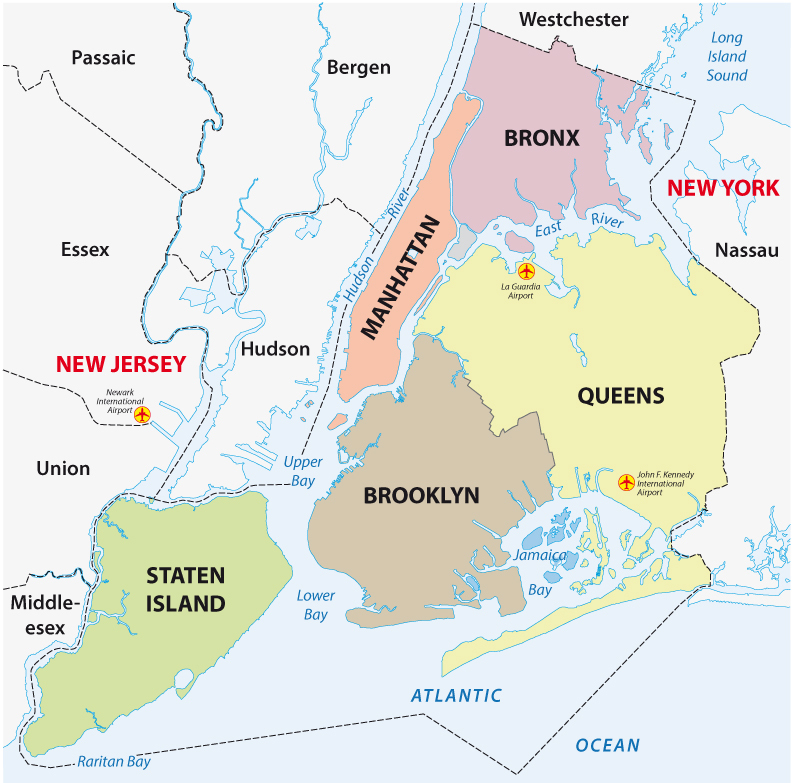
\includegraphics[width=.5\textwidth]{NYC_boroughs}
\end{center}


Linguistically:

\begin{itemize}
	\item No difference between accents in different boroughs.
	\item Problem: need to compare speakers of similar backgrounds from different boroughs; this comparison has not been done.
	\item Where do these perceived differences come from? New Yorkers conflate social class difference and their ideas about populations of boroughs. 
		\begin{itemize}
			\item Brooklynese: People with higher degree of presence of New York City English features are viewed as more ``working class,'' and New Yorkers tend to associate this dialect with Brooklyn --- traditionally, a working class borough on NYC.
		\end{itemize}
	\item Perception study: Can you identify which borough the dialect is from? Quiz is accessible at \url{http://www.newyorkcityaccents.com}.
		\begin{itemize}
			\item Results: New Yorkers cannot identify the borough from the accent.
			\item Listeners do not randomly guess: the distribution of answers is not uniform.
			\item Heavy New York accents are placed outside of Manhattan. 
			\item Voices with lower rates of classic NY City features are placed in Manhattan.
			\item No features distinguishing outer boroughs, i.e. Queens or Brooklyn.
			\item Class differences are important.
		\end{itemize}
 \end{itemize}

\section{Ethnicities in NY City}

\begin{itemize}
	\item In \citeposs{Labov:1966} study: Lower East Side: Jewish vs. Italians. Everyone is using the same dialect, but degrees differ.
	\item Currently, it is non-white speakers that maintain classical New York City features more, while white speakers lose these features at a greater rate.
	\item Interesting picture appears from considering Hispanics, African-Americans, Asians: this is currently the main locus of variability in NY City English. 
\end{itemize}

\section{Gender Influence}

\begin{itemize}
	\item Women are innovators, while men are more conservative.
	\item Women use more \emph{r}-ful pronunciations than men.
	\item Women withdraw from \emph{thought}-raising faster than men.
	\item It is possible that gender in such contexts is a byproduct of class	: ``how maleness intersects with working class identity."
\end{itemize}

\section{Using Language to Establish one's Social Identity}

Humans are social agents and play out their identity differently at different times.

\noindent Study of \emph{r}-lessness on Lower East Side (\citealp{Becker:2009}). 

\begin{itemize}
\item In conversation about local issues speakers use more r-lessness.
\item It enhances the message that speakers are trying to convey and reinforces the ``good old'' view of the local neighborhood.
\item Language change is used to reinforce certain ideas and evoke images in the conversation partner.
\end{itemize}

\section{Questions}

\begin{itemize}
\item From your experience, do you agree with the claim that boroughs do not have distinct accent?
\item Think about the different between the speech of your male friends and female friends. Do you notice any differences? Who speaks more standardly? Who uses more stigmatized features?
\item Which predictions can you make about the speech of people from different ethnic groups in NYC? Who would be speaking more standardly, White, African-American, Hispanic, or Asian New Yorkers? Why?
\item Do you or your friends chance the way they speak depending on a topic? Can you think of some examples?
\end{itemize}


\bibliographystyle{linquiry2}
\bibliography{../Bibliography/LIN200}

\end{document}
